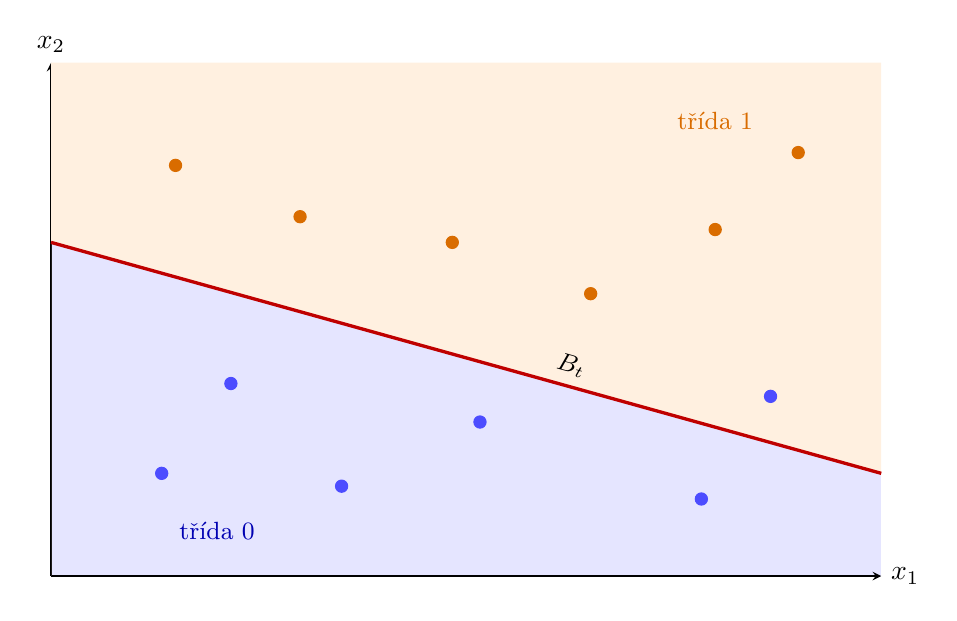
\begin{tikzpicture}
    \begin{axis}[
        width=\textwidth,
        height=8.1cm,
        xmin=0, xmax=6,
        ymin=0, ymax=4,
        axis lines=left,
        xlabel={$x_1$},
        ylabel={$x_2$},
        xtick=\empty,
        ytick=\empty,
        enlargelimits=false,
        clip=false,
        axis background/.style={fill=blue!10},
        every axis x label/.style={
            at={(current axis.right of origin)},
            anchor=west
        },
        every axis y label/.style={
            at={(current axis.above origin)},
            anchor=south
        }
    ]

        % oblast třídy 1
        \addplot[
            draw=none,
            fill=orange!12
        ] coordinates {
            (0,2.6)
            (6,0.8)
            (6,4)
            (0,4)
        } \closedcycle;

        % rozhodovací hranice
        \addplot[
            very thick,
            red!75!black,
            domain=0:6,
            samples=2
        ] {2.6 - 0.3*x}
        node[pos=0.62, above, sloped, black] {\small \(B_t\)};

        % body třídy 0
        \addplot[
            only marks,
            mark=*,
            mark size=2.2pt,
            blue!70
        ] coordinates {
            (0.8,0.8)
            (1.3,1.5)
            (2.1,0.7)
            (3.1,1.2)
            (4.7,0.6)
            (5.2,1.4)
        };

        % body třídy 1
        \addplot[
            only marks,
            mark=*,
            mark size=2.2pt,
            orange!85!black
        ] coordinates {
            (0.9,3.2)
            (1.8,2.8)
            (2.9,2.6)
            (3.9,2.2)
            (4.8,2.7)
            (5.4,3.3)
        };

        % popisky oblastí
        \node[blue!70!black, font=\small] at (axis cs:1.2,0.35)
            {třída~\(0\)};
        \node[orange!85!black, font=\small] at (axis cs:4.8,3.55)
            {třída~\(1\)};

    \end{axis}
\end{tikzpicture}
